\relatorio
{Análise Comportamental em Plataformas Digitais: Aplicando Cadeias de Markov e Simulações de Monte Carlo}
{
    \noindent Pesquisadores: Antônio Vicente Fernandes de Andrade, Rafael Albuquerque, João Pazotti    
}
{
    Este artigo apresenta um trabalho de consultoria realizado pela organização estudantil Insper Data para a empresa FRST - Falconi. O objetivo da análise foi entender os padrões de comportamento dos usuários da plataforma online do cliente. As ferramentas utilizadas para esse fim foram a teoria das Cadeias de Markov e, paralelarmente, simulações de Monte Carlo. Como resultado da nossa análise conseguimos identificar os estados (áreas do site) mais relevantes para entender a dinâmica de engajamento do usuário, isto é, as páginas que mais reforçam ou diminuem o engajamento. Esse trabalho é muito relevante em paralelo ao time de produtos da FRST, que focarão no redesenho dos estados indicados.
}
{Cadeia de Markov, Simulação de Monte Carlo}

\section{Introdução}
Dado a nova dinâmica que a era digital trouxe, cada clique e interação geram dados, o que transforma cada janela de um site em uma rica fonte de informações. Esse ambiente gera, portanto, grandes oportunidade para entender o comportamento e as decisões dos usuários. 
Neste contexto, nosso estudo propõe-se a explorar esses padrões de comportamento na plataforma da FRST, um ambiente digital com um grande trafego de usuários, através da aplicação da teoria das Cadeias de Markov, que nos dão um amparo robusto para modelar processos estocásticos e, sobretudo, para entender o próximo estado que cada um dos clientes da FRST escolherão baseado no estado em que estão agora, e Simulações de Monte Carlo, que permitem a simulação de interações de usuários reais na plataforma, o que nos possibilitará identificar tendências que não são facilmente perceptíveis. 
O objetivo deste estudo é, então, empregar essas metodologias para identificar os estados que mais impactam os padrões de comportamento do usuário e sugerir para o time de produtos do parceiro um "ranking" de estados que mais necessitam de um redesenho.

\subsection{Sobre a FRST}
A FRST, uma filial do grupo Falconi, é uma plataforma focada no aprendizado através do  fomento a uma comunidade de resolução de problemas. A empresa, com mais de 1000 clientes e mais de 30 mil usuários tem como modelo de negócio promover um espaço no qual os usuários consigam tirar suas dúvidas através da criação de "Desafios" e da recomendação de trilhas de conteúdo educativo com base no perfil do sujeito. 
Cada Desafio segue o método científico e, uma vez que é publicado, a ideia é que outros usuários consigam interagir e compartilhar como resolveriam ou resolveram problemas semelhantes ao divulgado. Já as trílhas de conteúdo são recomendadas pela plataforma após o onboarding na plataforma, onde o usuário tem que fazer uma redação de "auto conhecimento". 

\section{Modelagem Teórica}
\subsection{Propriedade Markoviana}

Processos Markovianos são todos aqueles que, além de estocásticos, respeitam a chamada 'Condição Markoviana', segundo a qual o futuro da série analisada independe de qualquer evento anterior ao estado atual em que ela se encontra. 

\begin{equation}
    P(X_{n+1} = x | X_n = x_n, X_{n-1} = x_{n-1}, \dots, X_0 = x_0) = P(X_{n+1} = x | X_n = x_n)
    \label{eq:propriedade}
\end{equation}


A propriedade Markoviana pode ser representada pela equação \ref{eq:propriedade}, \cite{Ross97}, na qual $X_{n}$ representa um estado no passo $n$ e $x , x_n, x_{n-1}, ... x_0$ representam as probabilidades de transição desse estado. Não é difícil enxergar, portanto, que a probabilidade de ir ao estado $X_{n+1}$ não é alterada pelos estados anteriores ($X_{n-1}$) uma vez que depende apenas do estado atual ($X_n$).

\subsection{Cadeias de Markov}

Nesse sentido, quando uma série estocástica, além de respeitar a condição markoviana , é discreta, podemos classificar esse processo Markoviano como uma Cadeia de Markov, que pode ser representada, em uma versão simplificada, pela figura \ref{fig:cadeia_01}.
Toda cadeia é comoposta por 3 elementos principais: Estados $(S_i)$, ações (as setas de um estado a outro) e as probabilidades de transição $(a_{ij})$, que são as probabilidades de cada ação acontecer.


\begin{figure}[!h]
\graphicspath{{relatorios/grupo3/Imagens/}}
    \centering
    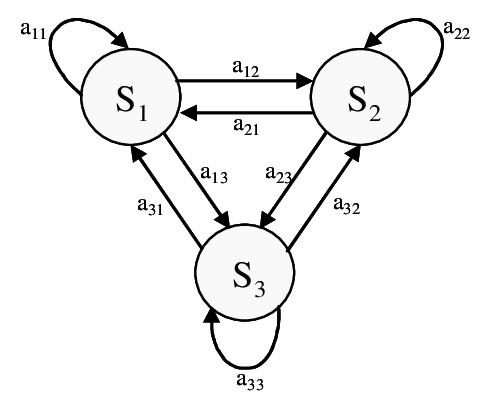
\includegraphics[width=0.5\linewidth]{A-Markov-chain-with-3-states.png}
    \caption{Cadeia de Markov com 3 estados}
    \label{fig:cadeia_01}
\end{figure}

As cadeias de Markov já são amplamente utilizadas em diversas áreas, como econometria financeira \cite{verhofen2005markov}, previsões temporais \cite{khiatani2017weather} e mecanismos de pesquisa e recomendação de conteúdo \cite{rai2016google}. Isso ocorre porque a, apesar de ser conceitualmente simples, a metodologia oferece uma grande adaptabilidade e robustez matemática. Em termos do nosso problema, podemos pensar em cada estado do site como a página de um site, com $S_1$ sendo o login, $S_2$ o menu e $S_3$ a área de desafios da FRST, por exemplo. Ainda, as ações possíveis são as transições de uma página do site para outra.

\subsubsection{Probabilidades de Transição}

Um benefício central das cadeias são as probabilidades de transição em sí. A perspectiva que as cadeias markovianas trazem, de que o passo seguinte depende apenas do presente e das probabilidades de transição atreladas a ele, nos ajuda a observar de forma intuitiva um problema de grande complexidade, que é a "previsão" das escolhas de terceiros. 

Uma forma de complementar a representação é montar uma  matriz com as probabilidades de transitar entre os estados, que recebe o nome de matriz de transição \ref{tab:matriz-de-transicao}. A partir dela, podemos aplicar ferramentas de álgebra linear e da propria teória Markoviana para extrair informações valiosas do problema. 

\begin{table}[h]
\centering
\caption{Matriz de Transição}
\[
P = \left( \begin{array}{ccc}
a_{11} & a_{12} & a_{13} \\
a_{21} & a_{22} & a_{23} \\
a_{31} & a_{32} & a_{33} \\
\end{array} \right)
\]
\label{mat:matriz-de-transicao}
\end{table}

\subsubsection{Probabilidades Estacionárias}

Um ponto que apesar de muito simples agrega muito à análise, são as probabilidades estacionárias. Essa probabilidades são um número fixo que representa a probabilidade de um usuário estar em um respectivo estado da plataforma após $n$ interações. Para chegar a essa matriz de probabilidades, elevamos a matriz de transição \ref{mat:matriz-de-transicao} a enesima potência \ref{eq:lim} e, em seguida, a pré-multiplicamos por uma matriz que representa o estado inicial do sujeito, ou \cite{Ross97} "Matriz de Decisão". Desse modo, chega-se ao vetor de probabilidades estacionárias $\pi$ \ref{eq:pi}. \cite{Ross97} 


\begin{equation}
S_0 = \begin{pmatrix}
s_{01} \\
s_{02} \\
s_{03} \\
\end{pmatrix}
\label{eq:s0}
\end{equation}

\begin{equation}
\lim_{n \to \infty} E = \lim_{n \to \infty} P^n \times \begin{pmatrix}
s_{01} \\
s_{02} \\
s_{03} \\
\end{pmatrix} = \pi
\label{eq:lim}
\end{equation}

\begin{equation}
\pi = \begin{pmatrix}
\pi_1 \\
\pi_2 \\
\pi_3 \\
\end{pmatrix}
\label{eq:pi}
\end{equation}

\subsection{Modelo MCMC (Markov Chain - Monte Carlo)}

Por fim, as cadeias possibilitam a criação de uma "Zona de Testes" que pode ser modificada da forma que o usuário preferir seja criando estados ou simulando a iteração de milhares de pessoas na plataforma com simulações de Monte Carlo.

As simulações de Monte Carlo são uma forma de resolver problemas utilizando uma "população hipotética" \cite{james1980monte}. A estratégia será utilizada aqui para simular os reais estados de saída dos usuários para buscar identificar as páginas que prejudiquem a experiência do cliente. 

\section{Dados e Modelagem Empírica}

\subsection{Adaptação de Estados}
As probabilidades de transição, representadas pelas linhas, indo de um estado a outro, foram calculadas com base em uma amostra com dados de navegação de clientes ao longo de 3 meses, somando aproximadamente 5000 sessões. Além disso, na base, temos o ID do usuário, o caminho que ele fez na plataforma e a data e o horário no qual ele entrou naquele estado.

A primeira etapa para começar a trabalhar com a base foi traduzir cada estado em um número de 0 a 22, ficando da seguinte forma:

\begin{description}
   \item[0] - Pesquisa Semântica.
   \item[1] - Opções Onboarding.
   \item[2] - (Modal) Cadastro de Desafio - Clique.
   \item[3] - (Modal) Cadastro de Desafio - Atualização
   \item[4] - Step 2 para o 3 do Onboarding
   \item[5] - (Modal) Cadastro de desafio - Mudança de Step
   \item[6] - Hall de Desafios
   \item[7] - (Modal) Cadastro de desafio - Listagem de Hipóteses
   \item[8] - Clique no botão para um desafio específico 
   \item[9] - (Modal) Cadastro de desafio - Upload de Arquivo
   \item[10] - (Modal) Cadastro de desafio - Ir de um formulário de desafio para outro.
   \item[11] - Hall de Desafios do usuário.
   \item[12] - Estado de Gerenciamento (Admin)
   \item[13] - Step 1 para o 2 do Onboarding
   \item[14] - (Modal) Cadastro de desafio - Cria um Indicador
   \item[15] - (Modal) Cadastro de desafio - Criar Desafio
   \item[16] - (Modal) Cadastro de desafio - Função para criar um Payload e cria um desafio
   \item[17] - Step 1 do Onboarding 
   \item[18] - Desabilita o Botão de Seguir 
   \item[19] - Clica nas notificações
   \item[20] - Clique no Menu Inicial
   \item[21] - (Modal) Cadastro de desafio - Função que inicia o desafio
   \item[22] - Login na Plataforma
 \end{description}

Além disso, representando nossa cadeia em um grafo, como foi feito anteriormente, na Figura 1, temos a visualização da Figura 2. Claramente a complexidade do problema é muito maior, dada a quantidade de relações entre cada estado.

\begin{figure}[!h]
\graphicspath{{relatorios/grupo3/Imagens/}}
    \centering
    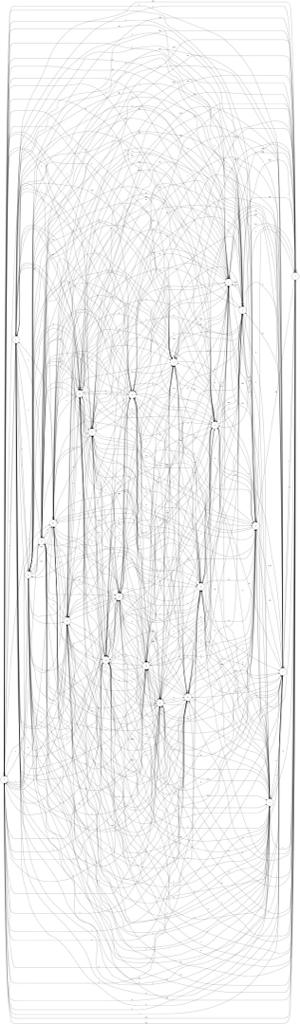
\includegraphics[width=0.25\linewidth, angle=90]{Grafo_FRST.jpeg}
    \caption{Cadeia de Markov FRST}
    \label{fig:enter-label}
\end{figure}

\subsection{Alterações na Base}

Foram feitas então duas modificações essenciais para o desenvolvimento da análise. A primeira foi adicionar, ao final de cada caminho de usuário, um novo estado, o 23º. Que representou o estado de saída do site. Essa modificação nos permite identificar quais são os estados que mais prejudicam o engajamento do usuário, dada a probabilidade de transição de cada estado para o fim do trajeto. A outra alteração foi garantir que cada caminho começará pelo estado 22, isto é, pela página de login do site. Essa alteração nos garantiu uma perspectiva mais clara das probabilidades de transição dado que todos "escolheram" começar pelo início do site.

\begin{table}[h] 
\centering
\begin{tabular}{l r r}
\hline
Id & Caminho Original & Caminho Novo\\
\hline
0 & [22][11][6][2] & [22][11][6][2][23] \\
1 & [7][2] & [22][7][2][23] \\
2 & [2][11][7][20] & [22][2][11][7][20][23] \\
\hline
\end{tabular}
\caption{Id e Trajetórias - Exemplo} % Adiciona a legenda
\label{tab:IdECaminhoOriginais} % Rótulo para referências cruzadas
\end{table}

\section{Resultados}
A abordagem aqui será muito simples. A ideia é observar as principais probabilidades estacionárias do site e compara-las com o fluxo efetivo de ida até o estado 23, encontrado através da simulação de Monte Carlo. Desse modo, se uma página do site tem uma alta probabilidade de presença e baixa probabilidade de transição para a saída, temos que essa página mantém o engajamento do usuário e abre espaço para mudanças e anúncios mais efetivos. Por outro lado, uma página que tem grande propabilidade estacionária e também um grande fluxo de saída, podemos indicar para a FRST que esse estádo contribui negativamente para a experiência do usuário e necessita de um redesenho ou, eventualmente, menos possibilidades de transição para ele ao longo do percurso na plataforma.

Nessa perspectiva, as principais probabilidades estacionárias das páginas do site foram os 5 estados presentes na tabela \ref{tab:stationary_probabilities}, somando aproximadamente 90\% de probabilidade das probabilidades de presença.

\begin{table}[ht]
\centering
\begin{tabular}{cc}
\hline
Estado & Probabilidade Estacionária (\%)\\ \hline
7 & \(30,1\) \\
2 & \(26,4\) \\
20 & \(19,7\) \\
6 & \(7,4\) \\
11 & \(4\) \\ \hline
\end{tabular}
\caption{Principais probabilidades estacionárias}
\label{tab:stationary_probabilities}
\end{table}

Como podemos observar, apesar das grandes probabilidades estacionárias dos estados ma tabela \ref{tab:stationary_probabilities}, apenas o estado 20 apresenta também uma grande representatividade na probabilidade de transicão para o estado 23 na simulação. O que pode indicar para a FRST que o Menu Inicial pode prejudicar o engajamento. 

\begin{table}[h]
\centering
\begin{tabular}{cc}
\hline
Estado & Percentual de Representatividade (\%) \\ \hline
20     & 29.01                                \\
19     & 23.70                                \\
11     & 19.95                                \\
9      & 13.20                                \\
12     & 5.17                                 \\
6      & 2.26                                 \\
0      & 1.84                                 \\
15     & 1.44                                 \\
2      & 1.38                                 \\
18     & 1.12                                 \\
10     & 0.37                                 \\
21     & 0.22                                 \\
7      & 0.22                                 \\
1      & 0.08                                 \\
5      & 0.03                                 \\
4      & 0.01                                 \\ \hline
\end{tabular}
\caption{\% de ida ao Estado 23 - Monte Carlo}
\label{tab:montecarlo}
\end{table}

\section{Próximos Passos}
Apesar de esse trabalho ter focado apenas na transição de um estado a outro, idealmente ele servirá de base para uma futura análise dos eventos criados por cada transição. Isto é, cada clique e interação dentro de cada página. De modo que buscaremos entender com maior profundidade o que cada usuário busca fazer na plataforma.  

\printbibliography[keyword = {markov}]
